\documentclass[twocolumn,a4,notitlepage]{report}

\usepackage[dvips]{graphicx}
%\usepackage{listings}
%\usepackage{url}
\usepackage{subfigure}

\include{epsf}

\title{
Amphisb\ae na \& Gorgophone\\
\includegraphics[width=10cm,height=10cm]{figures/amphisbaena.ps}\\
Simulating Various Morphologies \& \\
Associated Charge-Transport\\ 
in Blends of Conjugated Polymers\\
With Application to Organic Solar Cells\\
\medskip
EXSS Summer UROP Project 2005
}
\author{Student: Jarvist Moore Frost\\
(email: {\tt jarvist.frost@ic.ac.uk}\\
Supervisor: Dr Jenny Nelson\\
(email: {\tt jenny.nelson@ic.ac.uk})
}
\begin{document}

\maketitle

\chapter{Amphisb\ae na: Polymer Reptation}

\section{Slithering Snake Algorithm}
Morphologies were generated by use of a two-headed Slithering-Snake monte carlo method.
A population of conjugated polymer chains (snakes) were drawn from a
Gaussian distribution of chain length with associated parameters $\bar{l}$ \&
$\sigma_l$, and then laid down randomly in the 3D lattice.

These polymer chains were constricted to move linearly, with one of the
heads extending itself by one unit in any of the three cartessian
directions. They were considered to be in a `sea' of other material, which
was displaced around the snake without energy cost.

For each `slither' of the monte-carlo simulation, a particular snake, head
and direction were chosen at random. A calculation was made of the energy
change associated with such a move, which came about as a result of the
interaction energies between lattice units of `snake' [conjugated polymer
oligomers] versus the sea' of other plastic or the snake material itself.
These energies were considered as occuring on cofacial lattice sites -
diagonal interactions were not considered.

Due to the constrictions placed on the snake movement, and once
consideration was made for the energy associated with a configuration where
a certain snake touched itself, this calculation could be simplified to a
energy summation over the lattice site that the `head' was about to move
into, and the site that the `tail' was about to depart from. This
calculation is independent of chain length.

When this energy, $dE$, was negative then the exothermic movement progressed
automatically. For $dE>0$, the endothermic movement progressed if there was
sufficient Boltzman energy to drive it

\subsection{Notes on Interaction Energies}

There are three interaction energies present in the simulation - that of
Snake-Snake, Sea-Snake (and therefore Snake-Sea) and Sea-Sea. However, it is
the relative energy between configurations that produces the morphologies,
and so all values were set to zero except for the Snake-Snake interaction
which was made positive for homophilic (clumping) morphologies, or negative
for heterophilic (lacework) morphologies. All three values remain varyable
however, to make it easier to repeat the simulations with realistic values.

The material was considered to sit in a non-interacting bounding box - i.e.
the interaction energy with the walls was zero for all materials. Without
writing any extension to the codes, it is possible to study the effect of
energetic interactions with a surface by simply varying the snake-snake
interaction energies.

\section{Implementation Details}

\subsection{Definition of a Slither}
Within the context of both the codes and this document, a `slither' is
considered to be an attempt to move a random snake in a random direction.
Therefore, if the randomly selected direction is found to be blocked or the
movement considered non-favourable, it is still counted as a slither.

\subsection{Scientifically Important Aspects}

Enabling the snakes to `follow their own tails' was found to be essential
for producing Homophilic morphologies that did not artificially solidify. As
a spiraled snake could follow itself around with no energy cost, it was
possible for `trapped' heads to have the freedom to move around \& reach
non-trapped location where the snake was once again capable of global moves.
This required a very small addition to the implementation - that the `tail'
of the snake was removed from the $3D$ matrix keeping track of lattice site
occupancies before the movement of the head was considered, with necessary
considerations for the $dE$ calculation \& consistency over time of the
lattice.

This, however, was the only `local move' that we included. A number of
papers highlight the importance of local moves (such as twists or kinks) in
allowing global behaviour to emerge and for the snakes to not get `stuck'.
However, it is never very clear exactly how much freedom the `global moves'
(slithers) have, with particular respect to the snakes being able to go
forwards \& backwards etc. 

The relationship between amount of local \& global moves does not effect the
eventual behaviour or morphologies, but only the rate at which the blends tend towards
equilibrium. And as none of the snakes became permanently stuck, I believe
that adding further local moves may increase the efficiency of the algorithm, but
should not effect the nature of the morphologies generated.

\subsection{Performance Important Aspects}

The snake segments were kept in a circular datatype ($oroborus$), with an
index integar pointing to the current `head' location. The head / tail
location changed as the snake reptated around the lattice.
This allowed snake
movements to involve a single memory write, rather than shuffling all
segments one unit. This kept snake movements time-constant with respect
to snake length, and order of magnitude faster than keeping the snakes in
linear arrays.

The $dE$ calculation is the core of the simulation, and it is essential that
it runs as fast as possible! A naive implementation would calculate the
total interaction energy of the snake in position $A$, then move the snake
and calculate the total energy of the snake in position $B$. However, as the
only energy changes occur at the `tail' \& `head' of the snake, it is
possible to just consider these segments. Special consideration
must be made of the case where the snake `touches' itself; namely that any
self-snake interaction energy changes must be counted twice - i.e. once for
the head touching the body, and once for the body touching the head. Again,
this refinement keeps the algorithm time-constant with respect to snake
length, and order-of-magnitude faster than the naive implementation.

\subsection{Current Performance \& Possibilities for Further Improvement}

The codes, as written, perform $>2$ Mega Slithers per second on a single
processor of a ``Sun Fire V250'' machine ($Grianan$) with a small lattice.
This figure drops to significently below $1$ Mega Slither for large lattices.

This difference is not algorithmic, but due to memory cache issues.
Currently the entire lattice is described by a block of $x,y,z$ addressed
memory. This means that the local-vicinity lookups used to calculate $dE$
result in looking across large distances in the address space for single values.
Discretising this block of memory into cubes of data would result in
significent speedup, as a whole block of information used to do the entire
$dE$ calculation would be read from slow heap memory into fast cache at
once.

The code currently spends nearly $50\%$ of its time running a
Mersenne-Twister pseudo-random number generator. This generator is
statistically clean for Monte-Carlo codes, and is both fast \& has a
suitably large period considering the consumption of random numbers.
However, the codes, as written, are rather inefficient in their consumption
of random numbers - for instance; a full sized random integar is consumed in
choosing one of 6 cartessean directions. Internally the Mersenne Twister
keeps a heap of random digits which are consumed \& generated as necessary,
so it should be possible to create bytewise \& bitwise access routines
to enable greater efficiency.

\section{Results}

\subsection{Equilibrium}

The equilibrium endpoint for homophilic snakes is clearly a full phase
seperation of the two polymers. However, it was noticed by studying a $2D$
morphology evolving against time, that there is an initial `local clumping'
phase where snakes form `islands' with their neighbours.

After the initial
formation of these islands, which have very low mobility with time themselves,
further aggregation of the material is by
periodically ejection of a few snakes (typically $1-3$) which are then free
to randomly walk around the lattice until being involved in another island.
The rate of such evaporation seems inversely dependent on size, and the
chance of a given island absorbing a certain randomly walking snake is
clearly postively dependent on the size of the island and therefore the
cross-section. Thereby, smaller islands were incorporated into the larger
ones, eventually forming a full phase seperation and the existance of just
one super-island.

The size of the initial clumps in the quasi-equilibrium were found to be
highly depedent on temperature. Too high a temperature would clumps from
forming, whereas too low would only enable very local and almost entirely
exothermic moves to occur - resulting in small disparate clumps forming. 

Total phase seperation requires many more orders of magnitude of time to
occur compared to interim local clumping. We believe that this interim stage
best describes experimentally produced solar cells, and that the annealing
stage could involve such temperature activated clumping.

\subsection{Percolation}

A function was written to check for percolating cluster. It was implemented
as a recursive algoritihm that electrified the bottom electrode, then caused
charge to transfer from face-connecting lattice sites. A measurement of the
fraction of snake sites as part of the percolating cluster connecting to the
bottom electrode was made. 

\begin{figure}[htb]
\centering
\label{percolate}
\includegraphics[width=5cm,angle=270]{figures/percolate.eps}
\caption{Figure displaying the fraction of segments connected to the base
electrode by a percolating cluster, versus the density of the mix, for
25-long chain pure blends of both homophilic \& heterophilic polymers.}
\end{figure}

Plotting this fraction against density of the mix [Fig. \ref{percolate}], it
became apparent that the heterophilic (lacework) blends met the 
percolation threshold at a lower density. The exact densities depended on the
nature of the blend, but such behaviour was exhibited by all sizes \& purity
of lengths studied.

\subsection{Simulation Parameters}

The largest homophilic clumps were found to be produced when
the $k_B T \approx E_{int}$, and as we were attempting to best distinguish
homophilic and heterophilic blends, this value was used throughout for all
simulations.

In terms of time to equilibrium, it would appear that most of the initial
clumping is done after $1-5 . 10^5$ slithers per snake, and so a figure
of $10^6$ slithers per snake was deemed sufficient to produce equilibrium
morphologies, and a figure of this magnitude was used for all production
runs of the codes.

\subsection{2D Morphologies}

The codes were adjusted to provide a live display of the reptation of small ($80x40$) 2D
morphologies in real time. This provided a very quick feed-back cycle for
tweaking simulation parameters. An output routine was written,
`print\_lattice\_pnm\_file' which outputed the snakes on the 2D lattice as a
greyscale bitmap with the tone representing the snake id [Fig. \ref{attractive_20}]. 
This could then be loaded into a photoeditor and have a
colour scale mapped onto the tones, producing colourful figures
[Fig. \ref{cattractive_20}] which showed the micro-morphology of the tangled snakes.

\begin{figure}[htb]
\centering
\subfigure [Homophilic (Clumping)]
{
\label{attractive_20}
\framebox{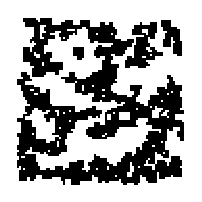
\includegraphics[width=5cm, angle=270]{figures/attractive_20.eps}}
}
\subfigure [Heterophilic (Lacework Pattern)]
{
\label{repulsive_20}
\framebox{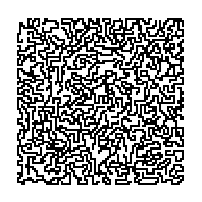
\includegraphics[width=5cm, angle=270]{figures/repulsive_20.eps}}
}
\caption{2D morphologies generated on a $80x80$ lattice using purely $25$ unit
snakes, at a $50\%$ by volume density. Simulations were run to
quasi-equilibrium. Identical simulation parameters were used for both,
except for the sign of the snake-snake affinity.}
\label{2d_morphology}

\end{figure}


\begin{figure}[htb]
\centering
\subfigure [Homophilic (Clumping)]
{
\label{cattractive_20}
\includegraphics[width=5cm]{figures/attractive_40pc_colour_morph.ps}
}
\subfigure [Heterophilic (Lacework Pattern)]
{
\label{crepulsive_20}
\includegraphics[width=5cm0]{figures/repulsive_40pc_colour_morph.ps}
}
\caption{
2D morpohologies generated on a $40x40$ lattice with a wide distribution
of snake lengths around an average of 25 units 
at $40\%$ volume density.
Colours were asigned to the different snakes at random, and are purely there
to indicate the micro-structre of the polymer chains. 
Identical simulation parameters were used for both,
except for the sign of the snake-snake affinity.}
\label{2d_morphology}

\end{figure}


\subsection{3D Morphologies}

The codes were always written for full 3D production, but with the unused
lattice dimension set to 1-unit for production of 2D data. 3D morphologies
produced significent visualisation problems, but attempts were made to
consider the morphology directly, rather than rely on numerical factors to
check approach to equilibrium.

\begin{figure}[htb]
\centering
\includegraphics[width=7.5cm]{figures/attractive_frame88.ps}
\medskip
\includegraphics[width=7.5cm]{figures/repulsive_frame88.ps}
\caption{Visualisation of $50x50x50$ 3D lattices by use of a denisity render
in $Povray$. The top cube represents homophilic (clumped) blends, brightness
indicates occupancy of `hoppers' during ToF simulation. The lower represents
a heterophilic (lacework) blend.}
\end{figure}

\subsection{Lattice `.dat' fileformat}

Due to the large times required to produce $1000x50x50$ lattices to
equilibrium, a fileformat was designed so that lattices could be stored on
disk \& then used for future studies.

The file is ASCII encoded, and is similar to the `pbm' ascii fileformat for
images. The first line contains four integars, $x \ y \ z \ num_{snakes}$
defining the lattice dimensions and maximum snakes. There
then follow $x * y$ lines of $z$ integars, which describe directly the
internal $lattice$ 3D integar array. These integars are either $-1$ to
describe an empty (sea) lattice site, or a postive integar (starting from
$0$, going to $num_{snakes}-1$) which gives the ID of the snake at that lattice site. The snake ID is
used in the CTRW program to detect when the snake is hopping to itself, with
a suitable consideration for the difference in intra and inter hop rates.

The functions `save\_lattice\_file' and `load\_lattice\_file' in
`lattice\_util.c' are used to save \& restore the lattices.

\chapter{Gorgophone: CTRW Time of Flight}

\section{CTRW Time of Flight}

\section{Implementation}

\subsection{Scientifically Important Aspects}

For the bulk of the simulations, using both $50x50x100$ and $50x50x1000$
sized lattices, a collection of 200 hoppers were run across the lattice at
one time. The hoppers blocked each other; if a site chosen by the CTRW was
occupied, a different site was chosen at random. Surrounding site's
occupency with hoppers did not effect total rate or associated wait time.

However, double-occupancy
of lattice sites could still occur by being `pipped at the post' by a
hopper already in the queue with the same destination.
In order to avoid this, a `ghost' hopper was placed in the
intended lattice site destination, which `reserved' the space for the
hopper. For the simplicity of the simulation, this was archieved by simply
having the hopper appear to occupy two sites at once - the current location
\& the preselected destination.

We used a value for site-reorganisation energy of $\lambda=0.5eV$, with no
disorder.


\subsection{Performance Important Aspects}

The most major cost of running this simulation was maintaining a queue /
fastest hopper selection process. If a ToF simulation where the hoppers were
transparent to each other (i.e. non-interacting) could be physically
justfied, far faster \& less complex codes could be written that just considered one hopper
at a time, averaged over many runs.

Homophilic (clumped) blends took a significently longer time to run a ToF
simulator over, due to the fact that the total hop rate in a clump was
significently faster due to the majority of the bounding sphere lattice
sites being occupied. This relative speed grew significently worse when
inter hops were made faster than intra hops, as in a 3D clump, a major
fraction of the snake is within the bounding sphere.

\subsubsection{Queue}

The hoppers were kept as an array of sorted `struct' items. As such,
inserting a hopper back into the queue once a wait time had been
recalculated was expensive in time. A linked list was considered to store
the hoppers, but would require the complexities of maintaining a lookup
table seperately in order to not simply shift the processing burden from
sorting the queue to traversing the list.

However, it was found to be quicker to allow the list to be semi-sorted.
Rather than resorting (via `qsort') the list everytime a hopper jumped, the
hopper was left in its current (now out of order) location, and the routine
used for selecting the hopper to jump checked iteratively through this
collection of unsorted hoppers \& the first item of the sorted queue to
select the one with the smallest wait time. Once the list was sufficiently
dirtied (and therefore the routine was having to check through a sufficient
number of hoppers), it was resorted.

With 200 hoppers, it was found that the fastest balance was to allow the
queue to become $\approx 70\%$ unsorted before requiring a resort.

The codes, as written, spend approximately $40\%$ of the time dealing with
the queue.

\subsubsection{Rate Tables}

It was found to be far faster to calculate the possible hop rates at the
start up of the ToF simulation, which was then used to populate a lookup
table for each lattice location. This was highly memory consuming, using
$700MB$ to store information for the $32$ potential hops of a $R_{Max}=2$
bounding sphere with a $1000x50x50$ lattice. However, it reaped a factor of
5 speed increase for the rate at which the Time of Flight simulation
progressed.

Clearly this would not be possible if the hoppers modified the local domain
(i.e. their electric charge effected the bias used to calculate other
hopper's jumps).

\section{Post Processing of Data}

\subsection{ToF fileformat}

$Gorgophone$ outputs to the stdout with a simple $ASCII$ fileformat
describing the time of flight. Initial lines consist of human readable
comments started with a `\#' character (which is ignored by the $gnuplot$
software used to generate the plots automatically). This is then followed by
blocks of ToF data with floating point values in three columns, which are
`bias time\_bin normalised\_current'.

\subsection{$\chi ^2$ Fitting of Transients}

In order to automate the generation of Pool-Frinkel plots, it was suggested
by `James Kirk-Patrick' to attempt a $\chi ^2$ fit of two lines against the
log-log scale transients. To this end,  codes were
produced with utilised the colourfully named `fit.c' linear fitting routine
from `Numerical Recipes'. 

Data is read in via `stdin', and is placed into an array of values. Current values
of less than $0.01$ are discarded as the transient is extremely noisy by that
point. The first point is also discarded; as this forms the entirity of the
initial `peak' before settling down onto the `shoulder' of the transient.

Fits are then attempted of the viable data, with a linear fit through the
first `n' data points, then a linear fit from that point to the end of the
viable data; with n constrained so that at least 3 data points were used for
both data points. The $\chi$ quality-of-fit values returned by the NR
routine were then scaled for the amount of data fitted by each line, and
compared to the minimum summated $\chi$'s so far. 

\chapter{Findings}

\section{Lattices}

A number of $1000x50x50$ blends were produced in the described fileformat,
which have been kept on file for future simulations, the most comprehensive
of which are for pure 25-length chains at a range of densities from $15-80\%$. For photocurrent
simulations \& other non-ToF simulations taking a smaller slice of the data
by reusing the access routines in `lattice\_util.c'.

\section{Non-discriminate Hopping Results}

\subsection{Effect of Morphology \& Bias on Transient Shape}


Heterophilic (lacework) morphologies were characterised by non-disperserve
charge-sheet like transport at low biases [Fig. \ref{repulsive_tof}], which were drawn out into
increasing dispersive transients as the bias increased. Higher density
blends produced higher mobilities, as expected, but also demonstrated
greater resistance to the bias-induced dispersion. I believe that such
behaviour can be described by the existence of physical fish-traps, where
the ToF hoppers are pulled downstream into non-percolating snakes. These
areas form physical traps into which the hoppers have to move against the
field gradient to escape. Higher densities of snakes produce greater
resistance to this due to the fact that the proportion of non-connecting
snakes will decrease as the density increases.

Homophilic (clumped) morphoogies produced generally dispersive transients
[Fig. \ref{attractive_tof}],
but which tended towards current-sheet behaviour for high densities.
Similarly, high biases resulted in increasing dispersive transport.

As the density approached $100\%$, the behaviour of both heterophilic \&
homophilic blends tended towards that of a pure sample - with entirely
current-sheet like transport with no bias-activated dispersion.


\begin{figure}[htb]
\centering
\subfigure [Homophilic (Clumping)]
{
\label{attractive_tof}
\framebox{\includegraphics[width=5cm,angle=270]{figures/a_0.25.bin_lattice.dat.ToF_trans.eps}}
}
\subfigure [Heterophilic (Lacework Pattern)]
{
\label{repulsive_tof}
\framebox{\includegraphics[width=5cm,angle=270]{figures/r_0.25.bin_lattice.dat.ToF_trans.eps}}
}
\caption{Simulated Time of Flights generated from $25\%$ density homophilic
\& heterophilic polymer blends. Current versus Time is presented on a
logscale, with the data collated into $150$ geometric timebins. Three biases
are displayed, $0.01, 0.05 \& 0.1 eV/site$.
}
\label{tofs}
\end{figure}

\subsection{Relative Mobility \& Pool-Frinkel Plots}

Due to the changing nature of the charge transport (non-dispersive becoming
dispersive at higher biases for homophilic clumped blends), Pool-Frinkel 
plots were of dubious use.

\subsection{Varying Polymer Chain Length}

Varying the polymer chain length was found to have 

\section{Snake ID Discrimination}

In order to study the effect of an increased rate of intra hops (between
oligomers of the same snake), a small change to the codes was made which
simply increased the tunneling rate if the material to be tunneled to was
represented as the same `id' as the current site.

This was a stop-gap measure, as a more physically correct model would be to
consider intra-hops as directly along the snake length. 

If one was studying a system where the intra hops could be considered to be
many orders of magnitude faster than inter hops, the setup can be considered
one where the electrons are distributed over the entire snake length, and
can hop from any lattice site with equal probability.

Although this would involve the calculation of a large number of possible
hops at the start of the simulation, these figures would be compiled down
into a single `ratetable' per snake, of which there are only thousands
rather than the millions of individual lattice sites. The ToF would benefit
from a considerable speedup.

\section{Conjecture}

The heterophilic (lacework) blends were demonstrated to have unique charge
transport properties, at least when intra-hops are sufficiently faster. The
lacework pattern itself leads to an extremely small diffusion distance for
exciton to reach a boundary, and enormous interfacial area. However, having
such tiny parallel running conduits for hole \& electron transfer is likely
to lead to a high level of recombination.

All the blend structure exhibited by the monte-carlo reptation occurs
through the interaction energies between the `heads' of the snakes. The
energies are also relative - one simply needs to consider the affinity of
the chain termination to the bulk polymer, versus that of the surrounding
sea of plastic. Stiff `needle-like' polymers might also be beneficial.

\end{document}
